\documentclass[a4paper]{tufte-handout}

% ams
\usepackage{amssymb,amsmath}

\usepackage{ifxetex,ifluatex}
\usepackage{fixltx2e} % provides \textsubscript
\ifnum 0\ifxetex 1\fi\ifluatex 1\fi=0 % if pdftex
  \usepackage[T1]{fontenc}
  \usepackage[utf8]{inputenc}
\else % if luatex or xelatex
  \makeatletter
  \@ifpackageloaded{fontspec}{}{\usepackage{fontspec}}
  \makeatother
  \defaultfontfeatures{Ligatures=TeX,Scale=MatchLowercase}
  \makeatletter
  \@ifpackageloaded{soul}{
     \renewcommand\allcapsspacing[1]{{\addfontfeature{LetterSpace=15}#1}}
     \renewcommand\smallcapsspacing[1]{{\addfontfeature{LetterSpace=10}#1}}
   }{}
  \makeatother

\fi

% graphix
\usepackage{graphicx}
\setkeys{Gin}{width=\linewidth,totalheight=\textheight,keepaspectratio}

% booktabs
\usepackage{booktabs}

% url
\usepackage{url}

% hyperref
\usepackage{hyperref}

% units.
\usepackage{units}


\setcounter{secnumdepth}{-1}

% citations
\usepackage{natbib}
\bibliographystyle{plainnat}


% pandoc syntax highlighting
\usepackage{color}
\usepackage{fancyvrb}
\newcommand{\VerbBar}{|}
\newcommand{\VERB}{\Verb[commandchars=\\\{\}]}
\DefineVerbatimEnvironment{Highlighting}{Verbatim}{commandchars=\\\{\}}
% Add ',fontsize=\small' for more characters per line
\newenvironment{Shaded}{}{}
\newcommand{\AlertTok}[1]{\textcolor[rgb]{1.00,0.00,0.00}{\textbf{#1}}}
\newcommand{\AnnotationTok}[1]{\textcolor[rgb]{0.38,0.63,0.69}{\textbf{\textit{#1}}}}
\newcommand{\AttributeTok}[1]{\textcolor[rgb]{0.49,0.56,0.16}{#1}}
\newcommand{\BaseNTok}[1]{\textcolor[rgb]{0.25,0.63,0.44}{#1}}
\newcommand{\BuiltInTok}[1]{#1}
\newcommand{\CharTok}[1]{\textcolor[rgb]{0.25,0.44,0.63}{#1}}
\newcommand{\CommentTok}[1]{\textcolor[rgb]{0.38,0.63,0.69}{\textit{#1}}}
\newcommand{\CommentVarTok}[1]{\textcolor[rgb]{0.38,0.63,0.69}{\textbf{\textit{#1}}}}
\newcommand{\ConstantTok}[1]{\textcolor[rgb]{0.53,0.00,0.00}{#1}}
\newcommand{\ControlFlowTok}[1]{\textcolor[rgb]{0.00,0.44,0.13}{\textbf{#1}}}
\newcommand{\DataTypeTok}[1]{\textcolor[rgb]{0.56,0.13,0.00}{#1}}
\newcommand{\DecValTok}[1]{\textcolor[rgb]{0.25,0.63,0.44}{#1}}
\newcommand{\DocumentationTok}[1]{\textcolor[rgb]{0.73,0.13,0.13}{\textit{#1}}}
\newcommand{\ErrorTok}[1]{\textcolor[rgb]{1.00,0.00,0.00}{\textbf{#1}}}
\newcommand{\ExtensionTok}[1]{#1}
\newcommand{\FloatTok}[1]{\textcolor[rgb]{0.25,0.63,0.44}{#1}}
\newcommand{\FunctionTok}[1]{\textcolor[rgb]{0.02,0.16,0.49}{#1}}
\newcommand{\ImportTok}[1]{#1}
\newcommand{\InformationTok}[1]{\textcolor[rgb]{0.38,0.63,0.69}{\textbf{\textit{#1}}}}
\newcommand{\KeywordTok}[1]{\textcolor[rgb]{0.00,0.44,0.13}{\textbf{#1}}}
\newcommand{\NormalTok}[1]{#1}
\newcommand{\OperatorTok}[1]{\textcolor[rgb]{0.40,0.40,0.40}{#1}}
\newcommand{\OtherTok}[1]{\textcolor[rgb]{0.00,0.44,0.13}{#1}}
\newcommand{\PreprocessorTok}[1]{\textcolor[rgb]{0.74,0.48,0.00}{#1}}
\newcommand{\RegionMarkerTok}[1]{#1}
\newcommand{\SpecialCharTok}[1]{\textcolor[rgb]{0.25,0.44,0.63}{#1}}
\newcommand{\SpecialStringTok}[1]{\textcolor[rgb]{0.73,0.40,0.53}{#1}}
\newcommand{\StringTok}[1]{\textcolor[rgb]{0.25,0.44,0.63}{#1}}
\newcommand{\VariableTok}[1]{\textcolor[rgb]{0.10,0.09,0.49}{#1}}
\newcommand{\VerbatimStringTok}[1]{\textcolor[rgb]{0.25,0.44,0.63}{#1}}
\newcommand{\WarningTok}[1]{\textcolor[rgb]{0.38,0.63,0.69}{\textbf{\textit{#1}}}}

% longtable
\usepackage{longtable,booktabs}

% multiplecol
\usepackage{multicol}

% strikeout
\usepackage[normalem]{ulem}

% morefloats
\usepackage{morefloats}


% tightlist macro required by pandoc >= 1.14
\providecommand{\tightlist}{%
  \setlength{\itemsep}{0pt}\setlength{\parskip}{0pt}}

% title / author / date
\title[分散の加法性を視覚的に理解する]{分散の加法性を視覚的に理解する}
\author{Sampo Suzuki, CC 4.0 BY-NC-SA}
\date{2021-06-01}

% --- 参考資料 ----------------------------------------------------------------
% https://github.com/Gedevan-Aleksizde/Japan.R2019/blob/master/latex/preamble.tex
% https://teastat.blogspot.com/2019/01/bookdown.html

% --- Packages ----------------------------------------------------------------
% 日本語とtufte, kableExtraを使うために必要なTeXパッケージ指定
% tufteではA4サイズの指定が不可能
%  A4 210mm x 297mm
%   \usepackage[a4paper, total={6.5in, 9.5in}]{geometry}
%   \usepackage{indentfirst}   # tinytexのリポジトリには存在しない?
% \usepackage[a4paper, total={160mm, 247mm}, left=25mm, top=25mm]{geometry}
% \usepackage[pdfbox,tombo]{gentombow}  % トンボを設定する場合は有効にする
\usepackage{ifthen}                     % 条件分岐用 \ifthenelse{条件}{T}{F}
\usepackage{booktabs}                   % ここからkableExtra用パッケージ
\usepackage{longtable}                  % 
\usepackage{array}                      % 
\usepackage{multirow}                   % 
\usepackage{wrapfig}                    % 
\usepackage{float}                      % 
\usepackage{colortbl}                   % 
\usepackage{pdflscape}                  % 
\usepackage{tabu}                       % 
\usepackage{threeparttable}             % 
\usepackage{threeparttablex}            % 
\usepackage[normalem]{ulem}             % 
\usepackage{inputenc}                   % 
\usepackage{makecell}                   % 
\usepackage{xcolor}                     % ここまでkableExtra用
\usepackage{amsmath}                    % 
\usepackage{fontawesome5}               % fontawesomeを使うために必要
\usepackage{subfig}                     % 複数の図を並べる際に必要(古い?)
% \usepackage{subcaption}                 % 同上(新しい?)
\usepackage{xeCJK}                      % 以下、日本語フォント用に必要
\usepackage[noto]{zxjafont}             % Linux環境ではこちを指定
% \usepackage[haranoaji]{zxjafont}      % Windows環境ではこちらを指定する
\usepackage{zxjatype}                   % 日本語処理に必要
\usepackage{pxrubrica}                  % ルビ用
\usepackage{hyperref}                   % ハイパーリンク用必要?

% --- Index ------------------------------------------------------------------
% https://texwiki.texjp.org/?%E7%B4%A2%E5%BC%95%E4%BD%9C%E6%88%90
% これを指定するとIndex(索引)は作成されるが参照ページがズレる
% 中間ファイルの.indではページはズレていないので、その後の結合処理がおかしい
% \usepackage{makeidx}
% \makeindex
% \usepackage{showidx}                  % 索引確認用

% --- Table of Contentes ------------------------------------------------------
% TOCにLOT(List of Tables), LOF(List of Figures), Bibliography, Indexを表示
% \usepackage[nottoc]{tocbibind}

% --- Fonts -------------------------------------------------------------------
% フォントしては index.html でも可能(pandoc用オプションは index.htmlにて)
% \setCJKmonofont{Source Han Code JP}
\setmonofont{Source Han Code JP}     % Linuxではこれのみコメントアウトする
% \setjamonofont{Source Han Code JP}

% ## 日本語フォントの扱いについてはzxjafontパッケージの解説を参照のこと
% # https://mirror.las.iastate.edu/tex-archive/language/japanese/zxjafont/zxjafont.pdf
% #
% ## Windows環境ではなぜかNotoフォントが認識されないので源ノシリーズベースの
% ## 原ノ味フォントかIPAexフォントを利用する(原ノ味はtlmgrでインストール可)
% # \usepackage[haranoaji]{zxjafont}
% # \usepackage[ipaex]{zxjafont}
% #
% ## Windows環境でNotoフォントを指定したい場合は以下のようにheader-includeで
% ## 個別に指定する(setCJKxxxfotnの指定は必要?)
% # \setmainfont{NotoSerifCJKjp-Regular.otf}[BoldFont=NotoSerifCJKjp-Bold.otf]
% # \setsansfont{NotoSansCJKjp-Regular.otf}[BoldFont=NotoSansCJKjp-Bold.otf]
% # \setmonofont{NotoSansMonoCJKjp-Regular.otf}[BoldFont=NotoSansMonoCJKjp-Bold.otf]
% ## モノフォントは源ノ角コード(Source Code Proの日本語版)がおすゝめ
% # \setmonofont{SourceHanCodeJP-Regular.otf}[BoldFont=SourceHanCodeJPS-Bold.otf]

\begin{document}

\maketitle




\hypertarget{introduction}{%
\section{\texorpdfstring{\textbf{Introduction}}{Introduction}}\label{introduction}}

 2021年度データ分析勉強会のテキストである『統計解析のはなし』\citep{ToukeiKaisekinoHanashi}の「標本が2つになれば」(P26〜)には分散の加法性の話が出てきます。分散の加法性は理解できるようでいて、理解できていないので、\textbf{R}を使って分散の加法性を可視化しながら説明してみます。

以降、平均値\(\mu\)、標準偏差\(\sigma\)、分散\(\sigma^2\)である正規分布を\(N(\mu, \sigma^2)\)と表記します。

 

\hypertarget{ux52a0ux6cd5ux6027ux3092ux53efux8996ux5316ux3059ux308b}{%
\section{\texorpdfstring{\textbf{加法性を可視化する}}{加法性を可視化する}}\label{ux52a0ux6cd5ux6027ux3092ux53efux8996ux5316ux3059ux308b}}

 以下の平均値と標準偏差を持つ二つの正規分布を\texttt{rnorm()}関数による正規分布乱数を用いて作成\footnote{n
  = \ensuremath{5\times 10^{6}}個の値を作成しています}します。

\begin{longtable}[]{@{}lccl@{}}
\caption{二つの正規分布}\tabularnewline
\toprule
正規分布 & 平均 & 標準偏差 & 備考 \\
\midrule
\endfirsthead
\toprule
正規分布 & 平均 & 標準偏差 & 備考 \\
\midrule
\endhead
\(N(\mu_a, \sigma^2_a)\) & \(\mu_a = 10\) & \(\sigma_a = 10\) & \\
\(N(\mu_b, \sigma^2_b)\) & \(\mu_b = 30\) & \(\sigma_b = 10\) & \\
\bottomrule
\end{longtable}

\begin{Shaded}
\begin{Highlighting}[numbers=left,,]
\NormalTok{a }\OtherTok{\textless{}{-}} \FunctionTok{rnorm}\NormalTok{(n, }\AttributeTok{mean =} \DecValTok{10}\NormalTok{, }\AttributeTok{sd =} \DecValTok{10}\NormalTok{)}
\NormalTok{b }\OtherTok{\textless{}{-}} \FunctionTok{rnorm}\NormalTok{(n, }\AttributeTok{mean =} \DecValTok{30}\NormalTok{, }\AttributeTok{sd =} \DecValTok{10}\NormalTok{)}
\end{Highlighting}
\end{Shaded}

\begin{marginfigure}

{\centering 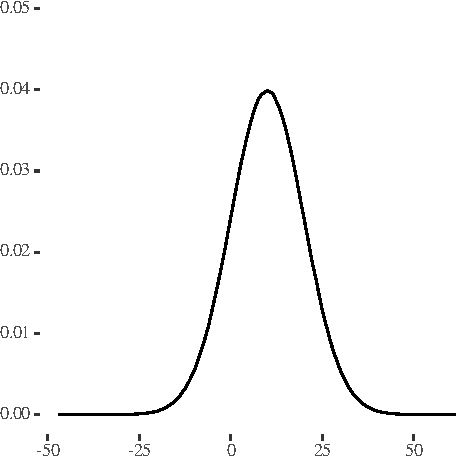
\includegraphics{AdditivityOfVariance_files/figure-latex/unnamed-chunk-2-1} 

}

\caption[$N(\mu_a, \sigma^2_a)$の分布]{$N(\mu_a, \sigma^2_a)$の分布}\label{fig:unnamed-chunk-2}
\end{marginfigure}

\begin{marginfigure}

{\centering 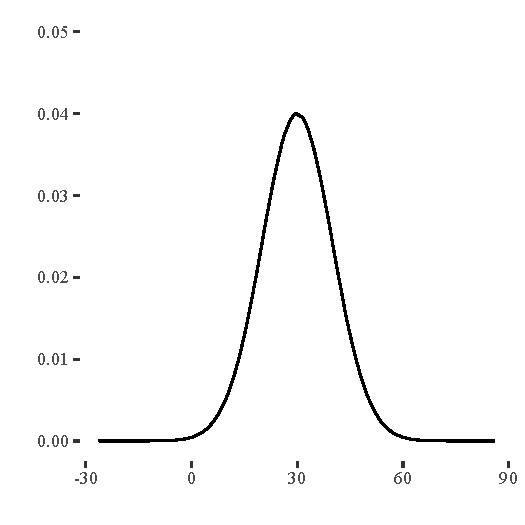
\includegraphics{AdditivityOfVariance_files/figure-latex/unnamed-chunk-3-1} 

}

\caption[$N(\mu_b, \sigma^2_bb)$の分布]{$N(\mu_b, \sigma^2_bb)$の分布}\label{fig:unnamed-chunk-3}
\end{marginfigure}

\begin{longtable}[]{@{}lcccl@{}}
\caption{二つの正規分布の要約統計量}\tabularnewline
\toprule
正規分布 & 平均 & 分散 & 標準偏差 & 備考 \\
\midrule
\endfirsthead
\toprule
正規分布 & 平均 & 分散 & 標準偏差 & 備考 \\
\midrule
\endhead
\(N(\mu_a, \sigma^2_a)\) & 9.9985888 & 99.9977663 & 9.9998883 & \\
\(N(\mu_b, \sigma^2_b)\) & 29.9965583 & 99.9706305 & 9.9985314 & \\
\bottomrule
\end{longtable}

この二つの正規分布\(N(\mu_a, \sigma^2_a)\)と\(N(\mu_b,\sigma^2_b)\)からランダムサンプリングにより一つずづ値を取り出して加算します。すなわち
 
\[N(\mu_a, \sigma^2_a)\mbox{ から取り出した値} + N(\mu_b,\sigma^2_b)\mbox{ から取り出した値}\]

という新しい値を作成します。取り出した値は元に戻し、同様の取り出し、加算を繰り返すと以下のようなデータが作成できます。ここではスペースの都合で先頭から限定して表示しています。

\begin{Shaded}
\begin{Highlighting}[numbers=left,,]
\NormalTok{c }\OtherTok{\textless{}{-}} \FunctionTok{c}\NormalTok{(}\FunctionTok{sample}\NormalTok{(a, n, }\AttributeTok{replace =} \ConstantTok{TRUE}\NormalTok{) }\SpecialCharTok{+} \FunctionTok{sample}\NormalTok{(b, n, }\AttributeTok{replace =} \ConstantTok{TRUE}\NormalTok{))}
\FunctionTok{head}\NormalTok{(c, }\DecValTok{50}\NormalTok{)}
\end{Highlighting}
\end{Shaded}

\begin{verbatim}
##  [1] 55.599241  5.237594 41.600298 23.359751 37.085258 44.437978  8.561242
##  [8] 20.376646 36.391691 50.055509 39.175702 23.941961 30.602629 33.448960
## [15] 32.419665 49.567928 39.905698 59.922084 63.553437  3.195873 25.325148
## [22] 38.901329 41.377471 57.117994 53.376228 63.967994 36.382754 61.459881
## [29] 35.738357 54.465682 73.874611 26.561265 55.829688 43.607332 56.616833
## [36] 51.793272 21.109510 40.752398 30.066753 63.453079 44.989330 52.826389
## [43] 34.170679 42.629914 30.266823 34.935418 55.543318 61.329707 63.234686
## [50] 67.256212
\end{verbatim}

分散の加法性により上記のデータは\(N(\mu_a + \mu_b, \sigma^2_a + \sigma^2_b))\)という正規分布になるはずですが実際はどうでしょう。各正規分布の平均値と分散を比較します。

\begin{longtable}[]{@{}lccl@{}}
\caption{各分布の要約統計量}\tabularnewline
\toprule
正規分布 & 平均 & 分散 & 備考 \\
\midrule
\endfirsthead
\toprule
正規分布 & 平均 & 分散 & 備考 \\
\midrule
\endhead
\(N(\mu_a, \sigma^2_a)\) & 9.9985888 & 99.9977663 & 元の分布 \\
\(N(\mu_b, \sigma^2_b)\) & 29.9965583 & 99.9706305 & 元の分布 \\
\(N(\mu_a + \mu_b, \sigma^2_a + \sigma^2_b))\) & 39.9951472 &
199.9683968 & 分散の加法性 \\
\(N(\mu_c, \sigma^2_c)\) & 40.0018296 & 199.9790041 & 実際の分布 \\
\bottomrule
\end{longtable}

このように確かに分散の加法性が成り立っており、正規分布\(N(\mu_a, \sigma^2_a)\)や\(N(\mu_b,\sigma^2_b)\)より横に広がった正規分布になっていることが分かります。

\begin{marginfigure}

{\centering 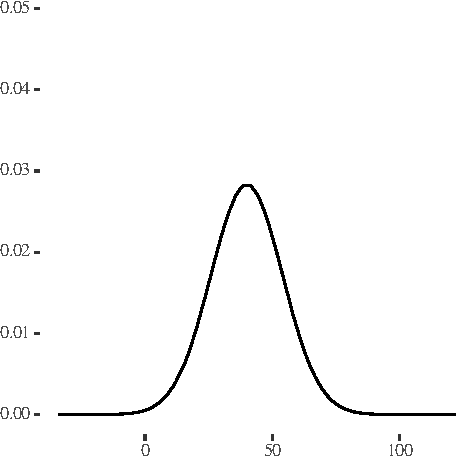
\includegraphics{AdditivityOfVariance_files/figure-latex/unnamed-chunk-5-1} 

}

\caption[$N(\mu_c, \sigma^2_c)$の分布]{$N(\mu_c, \sigma^2_c)$の分布}\label{fig:unnamed-chunk-5}
\end{marginfigure}

\newpage

\hypertarget{ux540cux4e00ux306eux6b63ux898fux5206ux5e03ux304bux3089ux53d6ux308aux51faux3057ux5024ux3092ux52a0ux7b97ux3057ux305fux5834ux5408}{%
\subsection{\texorpdfstring{\textbf{同一の正規分布から取り出し値を加算した場合}}{同一の正規分布から取り出し値を加算した場合}}\label{ux540cux4e00ux306eux6b63ux898fux5206ux5e03ux304bux3089ux53d6ux308aux51faux3057ux5024ux3092ux52a0ux7b97ux3057ux305fux5834ux5408}}

 次に二つの正規分布\(N(\mu_a, \sigma^2_a)\)と\(N(\mu_b,\sigma^2_b)\)がまったく等しいと仮定します。つまり

\[\mu_a = \mu_b = \mu_d\]

\[\sigma_a = \sigma_b = \sigma_d\]

という正規分布\(N(\mu_d, \sigma^2_d)\)を作成します。

\begin{Shaded}
\begin{Highlighting}[numbers=left,,]
\NormalTok{d }\OtherTok{\textless{}{-}} \FunctionTok{rnorm}\NormalTok{(n, }\AttributeTok{mean =} \DecValTok{10}\NormalTok{, }\AttributeTok{sd =} \DecValTok{10}\NormalTok{)}
\FunctionTok{head}\NormalTok{(d, }\DecValTok{50}\NormalTok{)}
\end{Highlighting}
\end{Shaded}

\begin{verbatim}
##  [1]  20.6262427  18.7804457   2.4013990   4.0130979  11.3286222   9.8768041
##  [7]   4.7568502   9.9090505  -4.0445735  16.5491671  20.6799970  12.4881164
## [13]   4.0029392  10.0473607  14.8913675  18.7336644  21.2705317  13.9545623
## [19]  14.4062801  12.8104317  26.6215824  29.2233908  24.3489912  -9.0156795
## [25]   8.8831009  -7.5751283  29.5895387   5.3455020  13.8686233  12.1810300
## [31]  -4.4800935   8.5103878  15.2268517  -5.5262560  11.7653608   8.7079841
## [37]  15.8605852   8.0033821  27.2542045 -12.9758471  16.5038052  10.0209208
## [43]  20.5733627  39.4137038  14.7399978  -1.0212168  -0.3178018  15.1327986
## [49]  15.6217370  22.2421247
\end{verbatim}

この正規分布\(N(\mu_d, \sigma^2_d)\)から先程と同様にランダムサンプリングにより一つずづ値を取り出して加算しますが、今回は同一正規分布\(N(\mu_d, \sigma^2_d)\)ですので、二つ取り出します。取り出した値は元の正規分布に戻し同様の操作を繰り返します。

 

\begin{Shaded}
\begin{Highlighting}[numbers=left,,]
\NormalTok{e }\OtherTok{\textless{}{-}} \FunctionTok{c}\NormalTok{(}\FunctionTok{sample}\NormalTok{(d, n, }\AttributeTok{replace =} \ConstantTok{TRUE}\NormalTok{) }\SpecialCharTok{+} \FunctionTok{sample}\NormalTok{(d, n, }\AttributeTok{replace =} \ConstantTok{TRUE}\NormalTok{))}
\FunctionTok{head}\NormalTok{(e, }\DecValTok{50}\NormalTok{)}
\end{Highlighting}
\end{Shaded}

\begin{verbatim}
##  [1] 37.037753 38.172461 19.844289 24.561710 34.982592 -9.961573 28.119099
##  [8] -5.797978 36.002053 39.808280 21.175291 41.142078 47.242403 17.248593
## [15] 14.811112 29.322576 40.337956 20.577689 -9.489254 30.694281 36.712260
## [22] 40.807344 27.422842 24.136736 37.564558  6.766611  3.815439 46.948949
## [29] 23.909628 42.335233 38.518215  8.076119 -3.642567 32.897224 31.090545
## [36]  8.275585 15.385796 12.435561 24.388711 19.495090 42.531706 33.668978
## [43] 24.224242 37.670191 31.613863 14.885696 36.773785 27.708292 30.518625
## [50] 26.337926
\end{verbatim}

\newpage

分散の加法性により以下が成り立ちます。

\[N(\mu_d + \mu_d, \sigma^2_d + \sigma^2_d) = N(2\mu_d, 2\sigma^2_d)\]

つまり、正規分布\(N(\mu_d, \sigma^2_d)\)から取り出した二つの値の和である正規分布\(N(\mu_e, \sigma^2_e)\)は

\begin{longtable}[]{@{}
  >{\raggedright\arraybackslash}p{(\columnwidth - 8\tabcolsep) * \real{0.16}}
  >{\centering\arraybackslash}p{(\columnwidth - 8\tabcolsep) * \real{0.20}}
  >{\centering\arraybackslash}p{(\columnwidth - 8\tabcolsep) * \real{0.20}}
  >{\centering\arraybackslash}p{(\columnwidth - 8\tabcolsep) * \real{0.36}}
  >{\raggedright\arraybackslash}p{(\columnwidth - 8\tabcolsep) * \real{0.09}}@{}}
\caption{加法性による要約統計量}\tabularnewline
\toprule
正規分布 & 平均 & 分散 & 標準偏差 & 備考 \\
\midrule
\endfirsthead
\toprule
正規分布 & 平均 & 分散 & 標準偏差 & 備考 \\
\midrule
\endhead
\(N(\mu_e, \sigma^2_e)\) & \(2 \mu_d\) & \(2 \sigma^2_d\) &
\(\sqrt{2 \sigma^2_d} = \sqrt{2}\sigma_d\) & \\
\bottomrule
\end{longtable}

という正規分布をすることになります。加法性と実際の正規分布を比べてみると

\begin{longtable}[]{@{}lccl@{}}
\caption{各分布の要約統計量}\tabularnewline
\toprule
正規分布 & 平均 & 分散 & 備考 \\
\midrule
\endfirsthead
\toprule
正規分布 & 平均 & 分散 & 備考 \\
\midrule
\endhead
\(N(\mu_d, \sigma^2_d)\) & 10.0045189 & 100.1240361 & 元の分布 \\
\(N(2\mu_d, 2\sigma^2_d)\) & 20.0090379 & 200.2480722 & 分散の加法性 \\
\(N(\mu_e, \sigma^2_e)\) & 19.9950719 & 200.0998858 & 実際の分布 \\
\bottomrule
\end{longtable}

となり、同一正規分布の場合でも分散の加法性が成り立っていることが分かります。

\begin{marginfigure}

{\centering 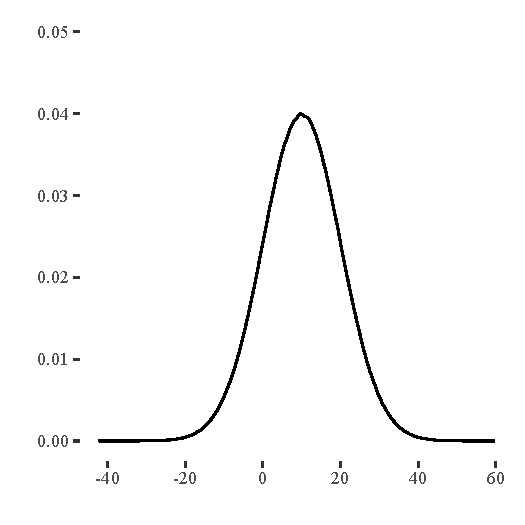
\includegraphics{AdditivityOfVariance_files/figure-latex/unnamed-chunk-8-1} 

}

\caption[$N(\mu_d, \sigma^2_d)$の分布]{$N(\mu_d, \sigma^2_d)$の分布}\label{fig:unnamed-chunk-8}
\end{marginfigure}

\begin{marginfigure}

{\centering 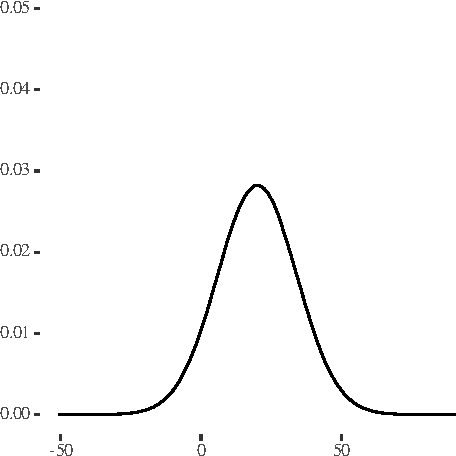
\includegraphics{AdditivityOfVariance_files/figure-latex/unnamed-chunk-9-1} 

}

\caption[$N(\mu_e, \sigma^2_e)$の分布]{$N(\mu_e, \sigma^2_e)$の分布}\label{fig:unnamed-chunk-9}
\end{marginfigure}

\newpage

\hypertarget{ux540cux4e00ux306eux6b63ux898fux5206ux5e03ux304bux3089ux53d6ux308aux51faux3057ux305fux5024ux3092ux5e73ux5747ux3057ux305fux5834ux5408}{%
\subsection{\texorpdfstring{\textbf{同一の正規分布から取り出した値を平均した場合}}{同一の正規分布から取り出した値を平均した場合}}\label{ux540cux4e00ux306eux6b63ux898fux5206ux5e03ux304bux3089ux53d6ux308aux51faux3057ux305fux5024ux3092ux5e73ux5747ux3057ux305fux5834ux5408}}

 同一の正規分布\(N(\mu_d, \sigma^2_d)\)から取り出した二つの値の\textbf{平均値の分布}を考えてみます。「二つの値の平均値の平均値」とは、正規分布\(N(\mu_d, \sigma^2_d)\)から、ランダムサンプリングで二つの値を取り出して、その平均値を取るということです。取り出した値は元の正規分布へ戻し、同様の操作を繰り返します。

\begin{Shaded}
\begin{Highlighting}[numbers=left,,]
\NormalTok{f }\OtherTok{\textless{}{-}} \FunctionTok{c}\NormalTok{((}\FunctionTok{sample}\NormalTok{(d, n, }\AttributeTok{replace =} \ConstantTok{TRUE}\NormalTok{) }\SpecialCharTok{+} \FunctionTok{sample}\NormalTok{(d, n, }\AttributeTok{replace =} \ConstantTok{TRUE}\NormalTok{)) }\SpecialCharTok{/} \DecValTok{2}\NormalTok{)}
\FunctionTok{head}\NormalTok{(f, }\DecValTok{20}\NormalTok{)}
\end{Highlighting}
\end{Shaded}

\begin{verbatim}
##  [1] 11.872711 22.680748  6.265354  7.445902 18.570496  7.158274 12.881660
##  [8] 18.359528 11.059736 16.541349  4.429276 -3.217499  1.008533  8.969713
## [15] 12.522954 16.699106  8.177954  9.148571 12.510590  4.637624
\end{verbatim}

この正規分布正規分布\(N(\mu_f, \sigma^2_f)\)は、二つの値の平均値、つまり二つの値を半分に割った値ですので正規分布\(N(2\mu_d, 2\sigma^2_d)\)のすべての値を半分にした正規分布になると予想できます。

\[\mbox{「二つの標本の平均値」の平均値} = \frac{2\mu_d}{2} = \mu_d\]

\[\mbox{「二つの標本の平均値」の標準偏差} = \frac{\sqrt{2}\sigma_d}{2} = \frac{\sigma_d}{\sqrt{2}}\]

\[\mbox{「二つの標本の平均値」の分散} = (\frac{\sigma_d}{\sqrt{2}})^2 = \frac{\sigma^2_d}{2}\]

\begin{marginfigure}

{\centering 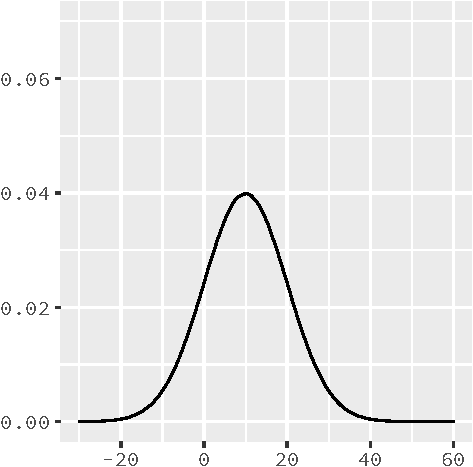
\includegraphics{AdditivityOfVariance_files/figure-latex/unnamed-chunk-11-1} 

}

\caption[$N(\mu_d, \sigma^2_d)$の分布]{$N(\mu_d, \sigma^2_d)$の分布}\label{fig:unnamed-chunk-11}
\end{marginfigure}

\begin{marginfigure}

{\centering 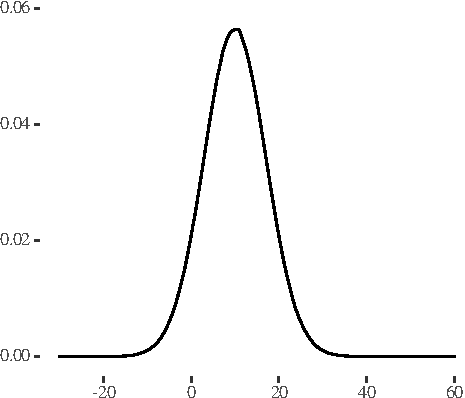
\includegraphics{AdditivityOfVariance_files/figure-latex/unnamed-chunk-12-1} 

}

\caption[$N(\mu_f, \sigma^2_f)$の分布]{$N(\mu_f, \sigma^2_f)$の分布}\label{fig:unnamed-chunk-12}
\end{marginfigure}

\begin{longtable}[]{@{}lcccl@{}}
\caption{各分布の要約統計量}\tabularnewline
\toprule
正規分布 & 平均 & 分散 & 標準偏差 & 備考 \\
\midrule
\endfirsthead
\toprule
正規分布 & 平均 & 分散 & 標準偏差 & 備考 \\
\midrule
\endhead
\(N(\mu_d, \sigma^2_d)\) & 10.0045189 & 100.1240361 & 10.0061999 &
元の分布 \\
\(N(\mu_d, \frac{\sigma^2_d}{2})\) & 10.0045189 & 50.0620181 & 7.0754518
& 分散の加法性 \\
\(N(\mu_f, \sigma^2_f)\) & 9.9998516 & 50.0590979 & 7.0752454 &
実際の分布 \\
\bottomrule
\end{longtable}

このように元の分布よりも鋭い分布になっていることがわかります。

\newpage

\hypertarget{ux4e09ux3064ux5024ux306eux5e73ux5747ux5024ux306eux5834ux5408}{%
\subsection{\texorpdfstring{\textbf{三つ値の平均値の場合}}{三つ値の平均値の場合}}\label{ux4e09ux3064ux5024ux306eux5e73ux5747ux5024ux306eux5834ux5408}}

 次に同一の正規分布\(N(\mu_d, \sigma^2_d)\)から取り出した三つの値の\textbf{平均値の分布}を考えてみます。
 

\begin{Shaded}
\begin{Highlighting}[numbers=left,,]
\NormalTok{g }\OtherTok{\textless{}{-}} \FunctionTok{c}\NormalTok{((}\FunctionTok{sample}\NormalTok{(d, n, }\AttributeTok{replace =} \ConstantTok{TRUE}\NormalTok{) }\SpecialCharTok{+} \FunctionTok{sample}\NormalTok{(d, n, }\AttributeTok{replace =} \ConstantTok{TRUE}\NormalTok{) }
        \SpecialCharTok{+} \FunctionTok{sample}\NormalTok{(d, n, }\AttributeTok{replace =} \ConstantTok{TRUE}\NormalTok{)) }\SpecialCharTok{/} \DecValTok{3}\NormalTok{)}
\FunctionTok{head}\NormalTok{(g, }\DecValTok{20}\NormalTok{)}
\end{Highlighting}
\end{Shaded}

\begin{verbatim}
##  [1] 10.898203 -1.444164 12.990511 16.287384  4.366764  9.781515  6.455512
##  [8]  8.475872  7.239857 10.628173  6.946945  5.182297 -0.421174 17.849796
## [15]  5.557278 20.180071 16.470020  9.177506 -4.355197 22.314048
\end{verbatim}

\begin{longtable}[]{@{}lcccl@{}}
\caption{各分布の要約統計量}\tabularnewline
\toprule
正規分布 & 平均 & 分散 & 標準偏差 & 備考 \\
\midrule
\endfirsthead
\toprule
正規分布 & 平均 & 分散 & 標準偏差 & 備考 \\
\midrule
\endhead
\(N(\mu_d, \sigma^2_d)\) & 10.0045189 & 100.1240361 & 10.0061999 &
元の分布 \\
\(N(\mu_g, \sigma^2_g)\) & 10.0074698 & 33.3804254 & 5.7775795 &
実際の分布 \\
比率 & 1.000295 & 0.3333907 & 0.5774 & 元の分布に対する比率 \\
\bottomrule
\end{longtable}

標準偏差の比率(0.5774)は、\(\frac{1}{\sqrt{3}} = 0.5773503\)とほぼ等しいことが分かります。これより

\[N(\mu_g, \sigma^2_g) = N(\mu_d, \frac{\sigma^2_d}{3})\]

となることがわかります。

\begin{marginfigure}

{\centering 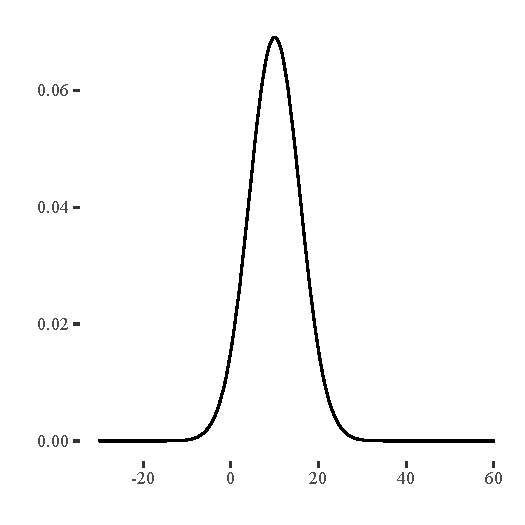
\includegraphics{AdditivityOfVariance_files/figure-latex/unnamed-chunk-14-1} 

}

\caption[$N(\mu_g, \sigma^2_g)$の分布]{$N(\mu_g, \sigma^2_g)$の分布}\label{fig:unnamed-chunk-14}
\end{marginfigure}

 

\hypertarget{ux4e00ux822cux5316ux3059ux308bux3068}{%
\subsection{\texorpdfstring{\textbf{一般化すると}}{一般化すると}}\label{ux4e00ux822cux5316ux3059ux308bux3068}}

 同一正規分布\(N(\mu, \sigma^2)\)から取り出した\(n\)個の値の\textbf{平均値の分布}\(N(\mu_, \sigma^2_n)\)は

\[N(\mu_n, \sigma^2_n) = N(\mu, \frac{\sigma^2}{n})\]

であり、平均は変わらず標準偏差が\(\frac{\sigma}{\sqrt{n}}\)となります。

\newpage

\hypertarget{cor.testux95a2ux6570ux306bux3064ux3044ux3066}{%
\subsection{\texorpdfstring{\texttt{cor.test()}関数について}{cor.test()関数について}}\label{cor.testux95a2ux6570ux306bux3064ux3044ux3066}}

 \texttt{cor.test()}関数は無相関の検定を行う関数です。対立仮説(\(H_1\))は下記の出力の通り「true
correlation is \textbf{not} equal to
0(相関係数はゼロではない)」ですので、帰無仮説(\(H_0\))は「相関係数はゼロである(相関はない)」となります。有意水準\(\alpha\)で検定が失敗すれば(帰無仮説が棄却されない、\(p \geqq \alpha\)である)帰無仮説が採択されますので相関係数はゼロ(データ間には相関がない)と考えられます。

\begin{verbatim}
## 
##  Pearson's product-moment correlation
## 
## data:  rnorm(n) and rnorm(n)
## t = 0.46846, df = 4999998, p-value = 0.6395
## alternative hypothesis: true correlation is not equal to 0
## 95 percent confidence interval:
##  -0.0006670199  0.0010860252
## sample estimates:
##          cor 
## 0.0002095028
\end{verbatim}

 

\hypertarget{appendix}{%
\section{Appendix}\label{appendix}}

\hypertarget{about-handout-style}{%
\subsection{About handout style}\label{about-handout-style}}

The Tufte handout style is a style that Edward Tufte uses in his books
and handouts. Tufte's style is known for its extensive use of sidenotes,
tight integration of graphics with text, and well-set typography. This
style has been implemented in LaTeX and HTML/CSS\footnote{See Github
  repositories
  \href{https://github.com/tufte-latex/tufte-latex}{tufte-latex} and
  \href{https://github.com/edwardtufte/tufte-css}{tufte-css}},
respectively.

 

\bibliography{bib/references.bib}



\end{document}
